\documentclass[10pt]{article}

\usepackage{amsmath}
\usepackage{amssymb}
\usepackage{anyfontsize}
\usepackage[toc,page]{appendix}
\usepackage{array}
\usepackage{authblk}
\usepackage{booktabs}
\usepackage{caption}
\usepackage{cellspace}
\usepackage{color}
\usepackage{enumerate}
\usepackage{enumitem}
\usepackage{fancyhdr}
\usepackage{float}
\usepackage{fontspec}
\usepackage{geometry}
\usepackage{graphicx}
\usepackage{listings}
\usepackage{multicol}
% \usepackage[skip=10pt plus1pt, indent=24pt]{parskip}
\usepackage{physics} 
\usepackage{sectsty}
\usepackage{subfigure}
\usepackage{tabularx}
\usepackage{unicode-math}
\usepackage{url}
\usepackage{wallpaper}
\usepackage{xeCJK} % chinese input

\setmathfont{XITS Math}
\setmonofont{Courier New}
\setmainfont{Times New Roman}
\setCJKmainfont{TW-Sung}

\renewcommand\thesection{\Roman{section}.}
\renewcommand\thesubsection{\normalsize \roman{subsection}.}
\sectionfont{\large \centering}
\subsectionfont{\centering \normalsize \it}

\geometry{
    a4paper,
    total = {170mm, 257mm},
    left = 15mm,
    right = 15mm,
    top = 18mm,
    bottom = 18mm
    }
\setlength{\lineskip}{3pt}
\setlength{\parskip}{3pt}

\definecolor{dkgreen}{rgb}{0,0.6,0}
\definecolor{gray}{rgb}{0.47,0.47,0.47}
\definecolor{mauve}{rgb}{0.478,0,0.82}
\lstset{frame = tb,
        language = Python,
        aboveskip = 3mm,
        belowskip = 3mm,
        showstringspaces = False,
        columns = flexible,
        basicstyle = {\small\ttfamily},
        numbers = left,
        numberstyle = \tiny\color{gray},
        keywordstyle = \color{blue},
        commentstyle = \color{dkgreen},
        stringstyle = \color{mauve},
        breaklines = true,
        breakatwhitespace = true,
        tabsize = 4}

\renewcommand\lstlistingname{Algorithm}
\captionsetup[lstlisting]{singlelinecheck=false, margin=12pt, labelsep=default, labelfont=default}
%We can also use: labelsep=period or labelsep=spacce, labelfont=default or labelfont=bf


%%%%%%%%%%%%%%%%%%%%%%%%%%%%%%%%%%% Again, Don't change anything Above %%%%%%%%%%%%%%%%%%%%%%%%%%%%%%%%%%%


\begin{document}


\pagestyle{fancy}
\fancyhf{} % clear all header and footer fields
\renewcommand{\headrulewidth}{0pt} %clear the header line 
\fancyhead[R]{
              \ifnum\value{page}>1 
              
\includegraphics[width = 0.2\textwidth]{nthu-logo.png} 
              \label{header}
              \else \fi
             }
\fancyfoot[C]{\thepage}

% title and info
\title{{\vspace{-2.5cm}
        \normalsize Computational Physics Lab - Final Report}\\
        \textbf{Common Prosperity}}
\author{Yuan-Yen Peng (彭元彥), Chih-Tian Ho(何之田)\\
        Advisor: Prof. Kuo-Chuan Pan(潘國全)}
\affil{\emph{Dept. of Physics, NTHU}\\
       \emph{Hsinchu, Taiwan}}
\date{\today}
\maketitle

\thispagestyle{fancy}

\setlength{\columnsep}{0.02\textwidth}
\begin{multicols}{2}

\section{Introduction}
    In the midterm, we desired to know whether quell the low class of people could haul up the entire echelon of humankind or not. However, in the wake of researching some literature, we find that useful and reliable references are too few to be applied. Then, we turn the rudder to focus on the simulation of the ring model compared to the real metropolitan city with different subsidized methods. 
         
    The principal purpose of this simulation is to investigate whether the hierarchy distribution in the ring model fits the metropolitan city. Since we can barely obtain data on popularity density distribution with high resolution, merely choosing to simulate the rank flows, we compare our consequences with house price distribution. Meanwhile, the simulation will utilize some physical functions and analogies to give a reasonable simulation.

\section{Methodology}
    
    \begin{figure}[H]
        \centering 
        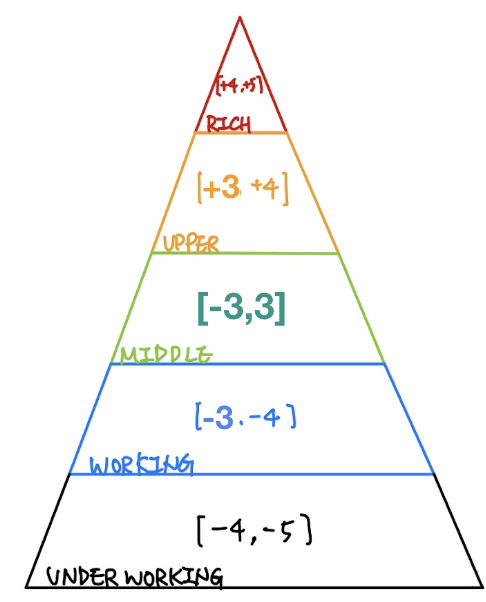
\includegraphics[width = 0.25\textwidth]{rank.png}
        \caption{This is the hierarchy pyramid. The number within the wedge corresponds to its social rank.}
        \label{rank}
    \end{figure}
    
    \subsection{Initial Setups}
        In this simulation, three parts need to be set up. First is the hierarchy, we classify the values of rank to the separated hierarchy, in Figure \ref{rank}. In addition, we set random ranks in the range of $[-3,3]$ in the grid (Figure \ref{ini_grid}, but we use $1000 \times 1000$ in the simulation) with the Dirichlet boundary condition of constant rank $-4$. Meanwhile, the main purpose of this simulation is to observe the rank distribution, in the other words, the population distribution is not the predominant target of this project. The second is the series of functions implemented to evolve the rank distribution at different times; besides, in the updated spin plan, we exploit the ``Jacobi-like'' method. The last is that we define maximum time ($t_{\text{max}}$) in $3 \times 4$ [years] with a week time split ($dt = 1\ \text{[week]}$)
    
    \begin{figure}[H]
        \centering 
        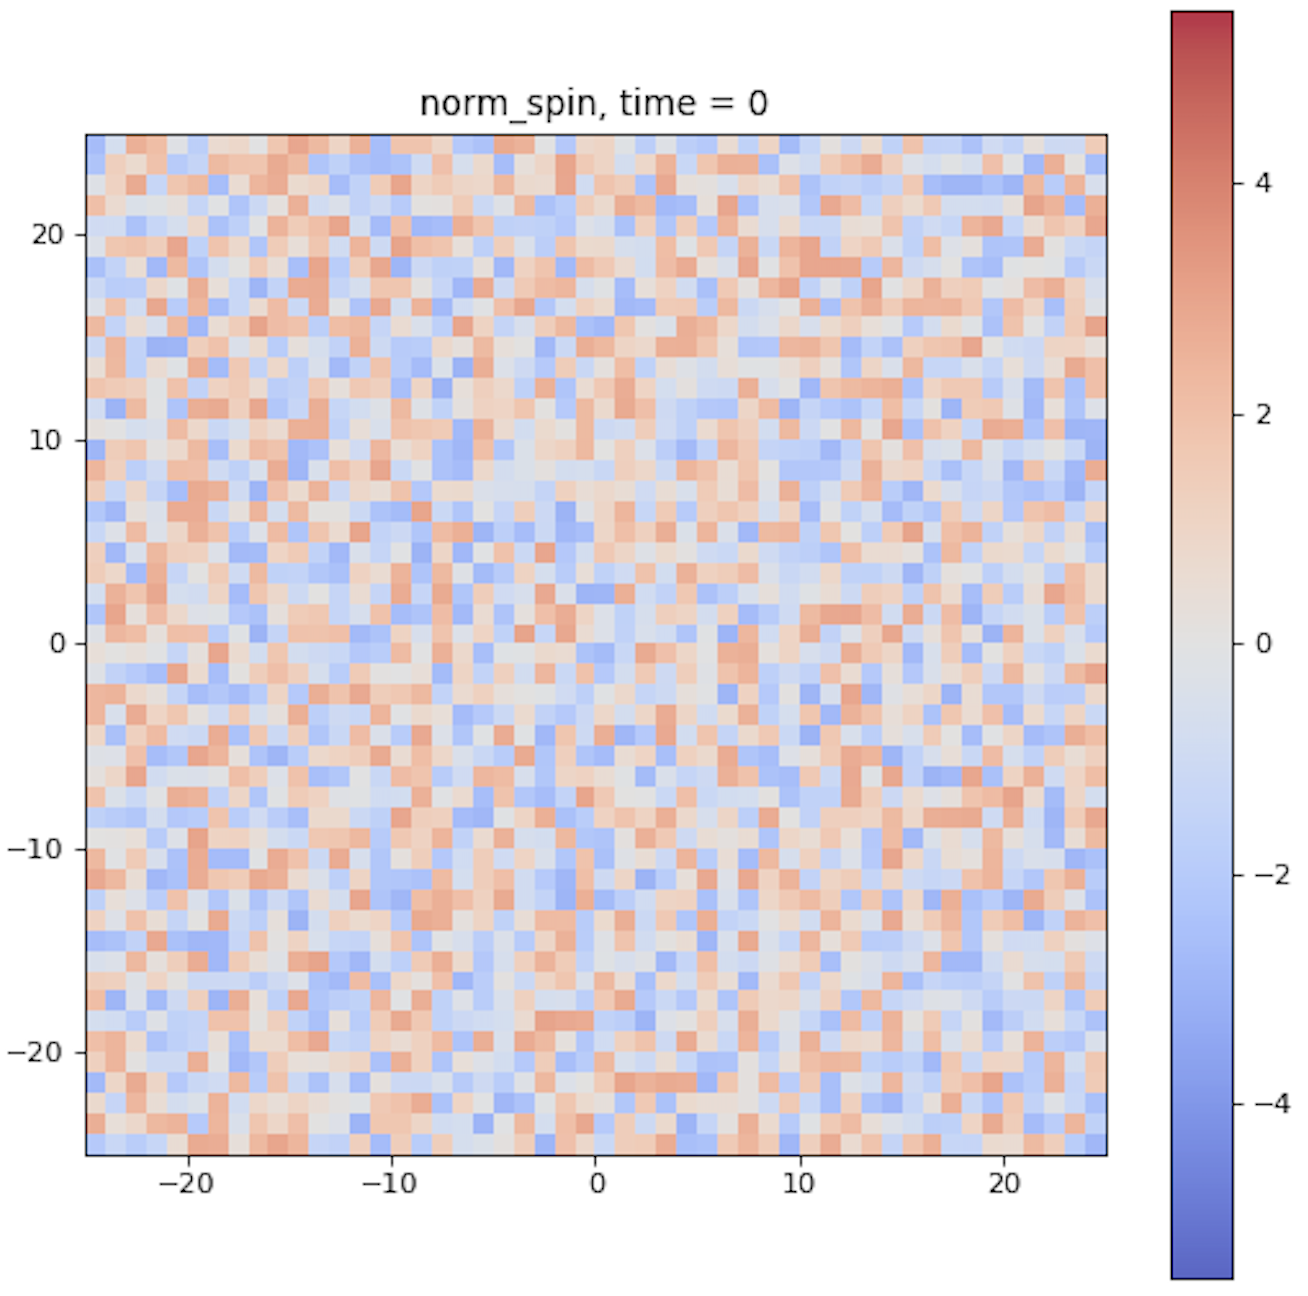
\includegraphics[width = 0.35\textwidth]{grid.png}
        \caption{This is the initial rank distribution with random hierarchy $[-3, 3]$ in the $50 \times 50$ grid. However, in the simulation, we use $1000 \times 1000$.}
        \label{ini_grid}
    \end{figure}
    
    \subsection{Exchange functions}
        The simulation will use some physical functions and analogies to give a reasonable consequence.

        Firstly, so as to distinguish the spin (rank) and a standard deviation; thus, we annotate the rank of each site as $H_{i,j}$.
            
        Then, we define the conduction function as Cond:
        \begin{align*}
            \text{Cond} = -\Big[  & (H_{i,j}-H_{i,j-1}) + (H_{i,j}-H_{i,j+1})   \\
                                  & + (H_{i,j} - H_{i-1,j}) + (H_{i,j} - H_{i+1,j}) \Big]
        \end{align*}
        The function describes the conduction between one site and its neighbors (above, below, left, and right). Since the hierarchy flow is from high to low, so there is a minus outside the sum of differences.

         We, next, define the absorbing function of conduction as Abs.cond:
        \[
            \text{Abs.cond} = \frac{1}{\sqrt{2 \pi a^2}} e^{-H_{i,j}^2 / 2 a^2}
        \]
        where $a$ is the standard deviation of all hierarchies, in our case, $a = 3$.
        This function is a normalized Gaussian distribution with mean = 0,and s.d. = 3, describing the absorbing rate of each site because the middle class ($[-3,3]$) has more desire for rank flow, note that we assume rank-0 has the most desire.

        Likewise, we define a background function as bkg (Figure \ref{bkg}):
        \[
            \text{bkg} = B \frac{1}{\sqrt{2 \pi a^2}} e^{- [\frac{(x - x_{mid})^2 }{2  \sigma_x^2 } + \frac{(y - y_{mid})^2}{2  \sigma_y^2 }]}
        \]
        where $B$ is a coefficient, in our case, $B \approx 8000$; $x_{mid}$ and ${y_{mid}}$ are the middle in the length and width, in our case, ${x_{mid}} = {y_{mid}} = 500$; $\sigma_x$ and $\sigma_y$ are the standard deviations of size, in our case, we set $\sigma_x = 0.1 \times \text{width} = 100$ and $\sigma_y = 0.1 \times \text{length} = 100$ depends on simulation results since we would get invalid results with a larger and smaller value. We assume the background function as a two-dimensional Gaussian distribution (exploit as a polar coordinate in the simulation) which describes that there is some resource that elevates every site's rank and contributes to overall social prosperity. 
        
    \begin{figure}[H]
        \centering 
        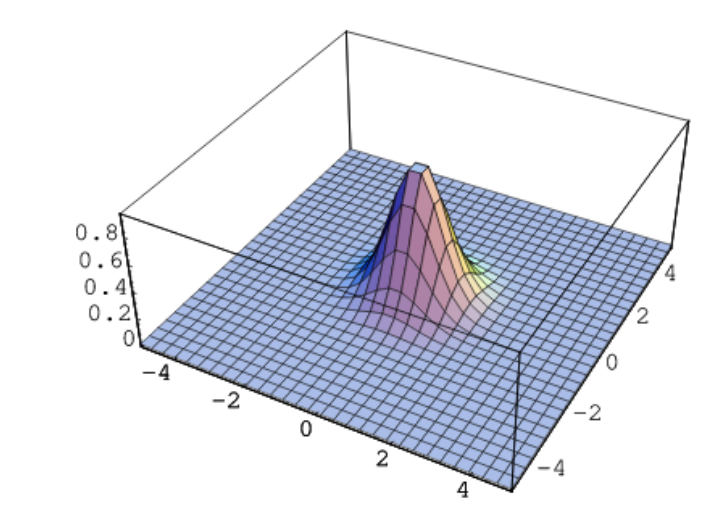
\includegraphics[width = 0.45\textwidth]{bkg.PNG}
        \caption{This is the plot of the background function at $t = 0$.}
        \label{bkg}
    \end{figure}

        In order to investigate the background source usage with time; thereby, we require the bkg to be a function of time and will be between [-1,1]. Hence, we need to let it times a time-depend function, here we choose a periodic function, prdc.func, sine, to simulate the condition:
        \[
            \text{prdc.func} = \sin (2\pi \times \frac{t}{t_{max}})
        \]
        where $t_{max}$ is the maximum time of our simulation.
        
        After that, we define the absorbing function of the background function as Abs.bkg(Figure \ref{abs.bkg}):
        \begin{align*}
            \text{Abs.bkg} = \eta \times (c_{1} e^{-5} e^{H} + c_{2} \frac{1}{\sqrt{2 \pi a^2}}  e^{-H^2 / 2 a^2})             
        \end{align*}
        where $c_{1}$ and $c_{2}$ are two simulated constants, which reflect the weightings of exponential and Gaussian terms, and in our case, we set $c_{1} = 0.05$ and $c_{2} = 0.95$, respectively; $\eta$ is the experimental constant, it describes the rate of usage of the background resource compared with conduction, in our case, $\eta = 0.07$ (for Beijing) This function tries to fit the absorbing rate of the background function, the former describes the more capable, the better able to take advantage of the environment; in general, the middle class has more desire for upgrading rank, so the latter describes its phenomenon.
    
        \begin{figure}[H]
            \centering 
            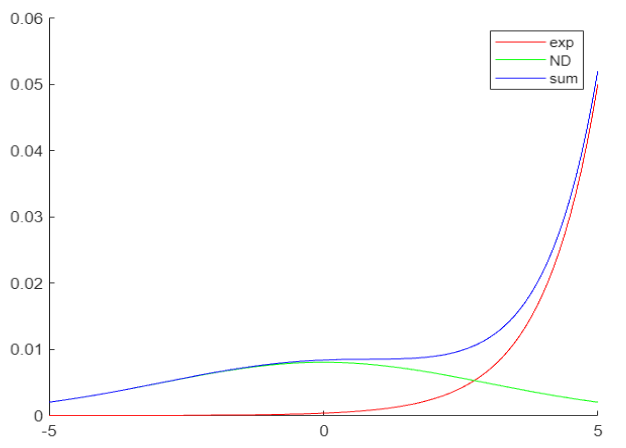
\includegraphics[width = 0.35\textwidth]{abs.bkg.PNG}
            \caption{Blue line is the plot of the absorbing function of the background function which is made up of red line(exponential) and green line(Gaussian).}
            \label{abs.bkg}
        \end{figure}

        We, therefore, combine all the functions shown above, obtaining the exchange function for iteration:
        \begin{align*}
            (\text{New\_H})_{i,j} & += 0.5 \times \text{Abs.cond} \times \text{Cond}\\
                                  & +  0.5 \times \eta \times \text{Abs.bkg} \times \text{bkg} \times \text{prdc.func}
        \end{align*}
        Additionally, there is a saying "The father buys, the son builds, the grandchild sells and his son begs." In the real world, it is common to see that rich families cannot hold their wealth, and successful people come from poor families, so we define two constant $p$ and $q$, which are the probabilities of rich to poor and poor to rich.

        By our reference \cite{3gen}, we want the survival rate of enterprise for three years is about 0.2, so we set both $p = q = 0.01$ for one week. Therefore, in our simulation:
        
        \noindent if $H_{i,j} > +5$,  by chance p:
        \begin{align*}
            & H_{i,j} = -4, \\
            & H_{i,j-1} = H_{i,j+1} = H_{i-1,j} = H_{i+1,j} ×= 0.3
        \end{align*}
        \noindent if $H_{i,j} < -5$, by chance q:
        \begin{align*}
            & H_{i,j} = +4, \\
            & H_{i,j-1} = H_{i,j+1} = H_{i-1,j} = H_{i+1,j} ×= 0.3
        \end{align*}


    \subsection{Subsidy Policy}
        In this section, we are going to see the difference in subsidy policy, here we choose two types of subsidy: equality and justice. Also, the purpose of the subsidy is to increase the prosperity of society, so the utility of the subsidy will be reflected in the rank of people.
        
        In general, equality refers to distributing subsidies evenly to everyone; justice indicates distributing subsidies to those who needed, see Figure \ref{toy}. In our simulation, we set the subsidy interval every three months and subsidized values are 0.01 and 0.02, respectively (because in this conditions of simulation, generally, we assign people who are in the whole rank $[-5,5]$, equality mode, will receive simply as twice as who are really in need, i.e., justice, which we set them in the $\text{rank} < 0$ in this project).

    \begin{figure}[H]
        \centering 
        
\includegraphics[width = 0.45\textwidth]{toy.png}
        \caption{The toy scheme for the definition of equality and justice \cite{toy}.}
        \label{toy}
    \end{figure}

    
    \subsection{Physical Analogy}
        In this project, we exploit four sorts of physical parameters to quantify the consequences of our simulation. First and foremost is spin, which is corresponding to social ranks. The second is the energy indicating social mobility, and we implement the ``Ising model like'' model to estimate the system's energy:
        \[
            E = -J\sigma_{i+1,j}\sigma_{i-1,j}\sigma_{i,j+1}\sigma_{i,j-1} - h\sigma_{i,j}
        \]
        where $J$ is the constant and here we simply set it to be positive because of the characteristic of paramagnetic, which we assume that the people will behave ``parallel'' in the people-people interactive; $h$ is the external field, which is related to the background function.

        The third is magnetization ($M$) and its average; that is magnetization per spin ($m$) representing the average social hierarchy. We utilize these to elaborate on the macro aspect of the system (not the site's local behavior).
        \[
            M = \sum \sigma_{ij}\ ;\quad m = \big\langle \sum \sigma_{ij} \big\rangle
        \]
        where $\sigma_{ij}$ means the site's spin (rank). We are, likewise, interested in the response to the dynamic in the phase space of $(m,h)$; thence, also implementing its ``response function'', susceptibility ($\chi$):
        \[
            \chi \equiv \frac{\partial m}{\partial h}
        \]
    
\section{Results}
    \subsection{City}
        \begin{figure}[H]
            \centering 
            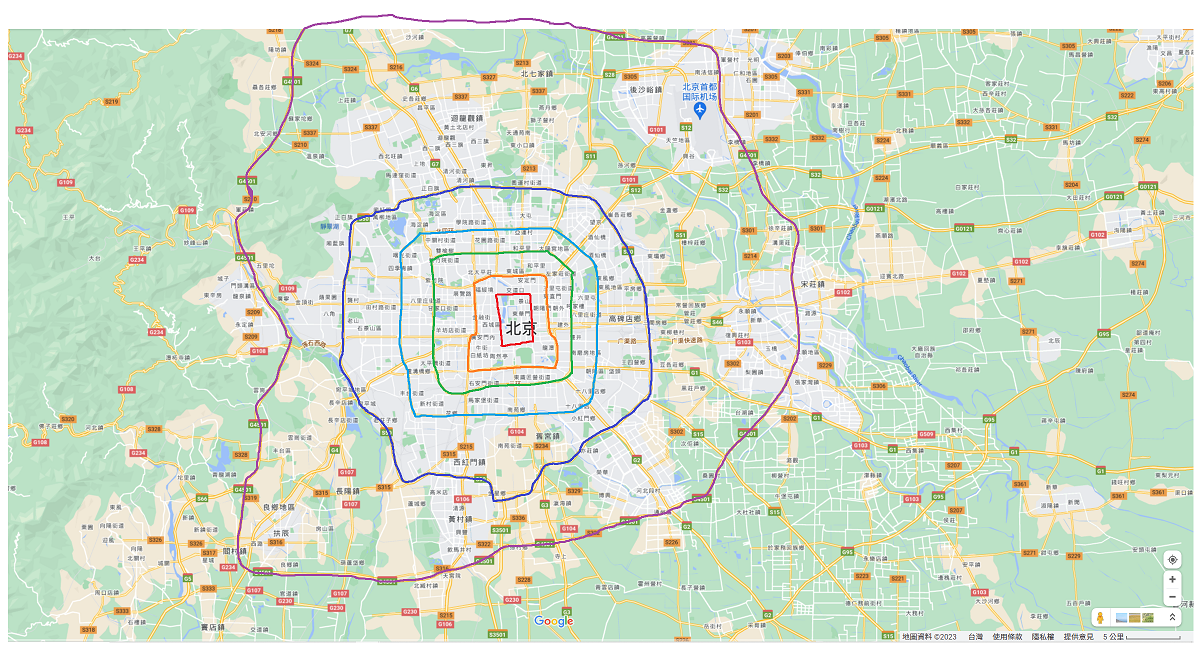
\includegraphics[width = 0.48\textwidth]{BeijingGoogle.PNG}
            \caption{This is the screenshot from Google Maps, and we mark the Six-rings environment(北京六環)with different colors.}
            \label{Google}
        \end{figure}
    
        In the map shown above, we choose Beijing as our fitting object since Beijing City is designed as a standard concentric structure, which is in line with the Burgess model (concentric zone model) theory \cite{ring_model}; also, in order to estimate the size of a site, we adopt the map scale in Figure \ref{Google}, getting the length and width of the sixth ring are both approximately $50 \text{[km]}$. Therefore, we set our site size of the grid to be $50\text{[m]} \times 50\text{[m]}$ (since our gird is $1000 \times 1000$), and then we overlay the screenshot with the simulated results as below:      

    \begin{figure}[H]
        \centering 
        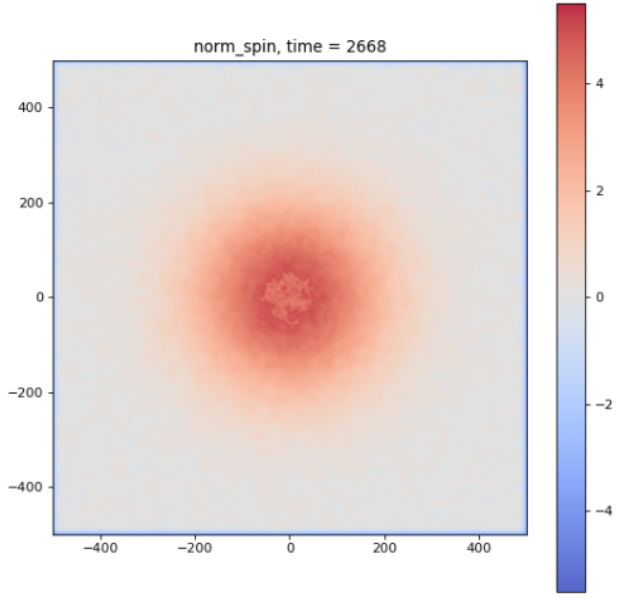
\includegraphics[width = 0.35\textwidth]{t=2668.PNG}
        \caption{We take a screenshot at $t = 2668 \text{[day]}$ from our simulation, indicating rank by color and the grid size is $1000 \times 1000,\quad (\text{i.e.,} \quad 50\text{[km]} \times 50\text{[km]})$ }
        \label{2668}
    \end{figure}

        We take a screenshot around $t_{max}/4$ since the distribution of rank is the most similar sample compared to the real case of Beijing City. There are some points worth observing: exists a small collapse in the center, and the max rank forms a ring around the center. Afterward, in order to investigate what is the real-world situation, we overlay our simulated outcome with Google Maps of Beijing City shown below:
        
    \begin{figure}[H]
        \centering 
        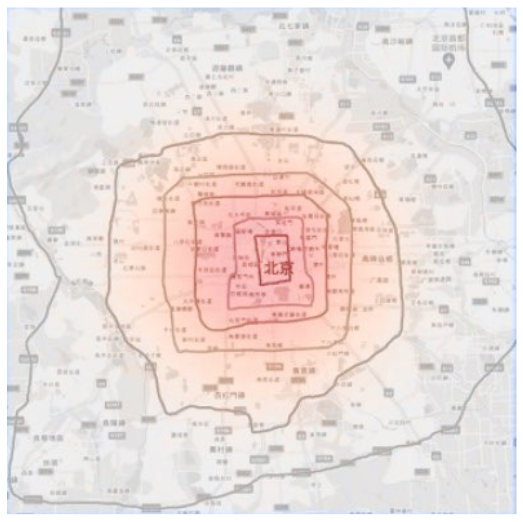
\includegraphics[width = 0.3\textwidth]{overlay.PNG}
        \caption{We overlay the screenshot (Figure \ref{2668}) with Google Maps (Figure \ref{Google}).}
        \label{overlay}
    \end{figure}
    
        From Figure \ref{overlay}, we can see the collapse locates inside the 1st ring, and the highest rank locates between the 1st ring and the 2nd ring. Moreover, around the 2nd to 5th rings, we can observe the rank decay with the distance, additionally almost no color outside the 5th ring. Hereafter, we can see how is the real house price distribution in Beijing City in Figure \ref{houseprice}.
        
    \begin{figure}[H]
        \centering 
        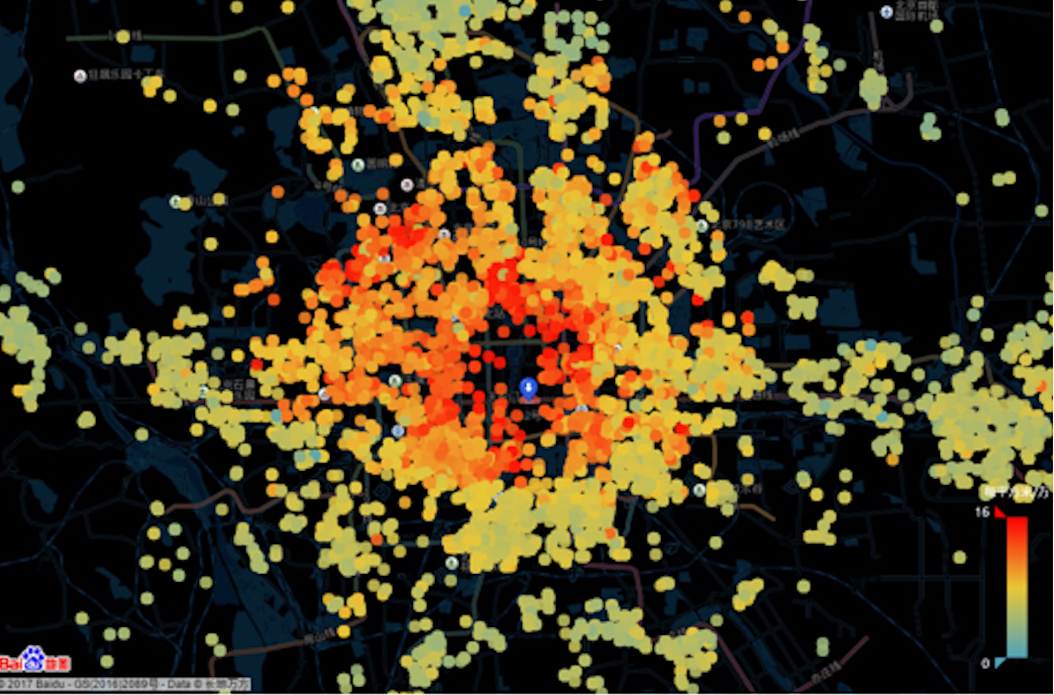
\includegraphics[width = 0.4\textwidth]{houseprice.PNG}
        \caption{This is the scatter plot of the house source data of $25,217$ second-hand housing data in Beijing on May 10, 2017, on \texttt{Lianjia.com}. According to the coordinates of the second-hand housing, which are the surrounding facilities data, including subways, buses, schools, and hospitals. \cite{price_git}}
        \label{houseprice}
    \end{figure}
    
        Figure \ref{houseprice} is a scatter diagram in the geographic coordinate space to display the housing price distribution in Beijing City. Each set of second-hand housing has corresponding coordinates (i.e., where the data is situated) and price data. Each set of second-hand housing mark as a point, and the color bar is on the bottom left corner. Although the quantity of the house price data is not sufficient enough and there are still many locations with no data, we can clearly see the distribution of real house prices is very similar to our simulation results. Because the highest rank lies between the 1st ring and 2nd ring, and the rank decay tendency with the distance around the 2nd to 5th ring is similar to our simulation's consequences. From the literature, \cite{new}, most of the people who are in the middle class and come to Beijing(北漂)is outside the 5th ring, and inside the 3rd ring is the ``high-class'' housing area, and the price will be higher when it approaches the center. However, because the central region is the most ``delicious zone'', so the government will take control of the area; that is, it will not partake in the free market. Thereby, we assert that the ``highest'' housing price might not situate in the center, instead, it might locate around the center. It seems like it fits our simulation consequence, but when we investigate deeply in our simulated process, we find that the detailed mechanism is not exactly the same in the central region.

        The small collapse in the center of the simulation results is an interesting phenomenon that we want to discuss. The main reason is that: at the beginning of the simulation, sites in the center region grow very fast since the background function contributed a lot, then the center keeps consuming more background resources owing to the large Abs.bkg in high rank. However, because of setting the upper-rank limit at +5, consuming background resources does not increase overall prosperity more in the center, so as time goes on, the probability of $p(\text{rich to poor})$ still affects the center. While there is no more background resource to support maintaining high ranks. Therefore, the system ends up with a small collapse in the center. Note that the probability of $p(\text{rich to poor})$ is more significantly effective in the center, and will transfer by conduction function in section Exchange functions. Compare to our simulation outcome, the tendency of this effect almost fits. Yet, the central region does not participate in the free market, we can just argue that the tendency excludes Beijing almost fits and if we want to completely research this model, we need to select another city that fully takes part in the free market.
    
    \subsection{Physical Analogy}
        On the heel of discussing the ``local'' behavior of the sites; that is city comparison, we are going to expound on the global behavior of the system. In Figure \ref{com}, the above shows the average magnetization vs external field. In the normal mode (red), there is a ``plateau'' around $1000 \sim 3300$ [code unit]; if we adopt subsidized methods, the plateau will rise, and in this condition (related to opportunity: here subsidy is 0.01/dt for both equality and justice in $0<\text{rank}$), the equality method will escalate most. 
        
        These outcomes illustrate that the average social rank will rise to a stable state (the social mobility will be low, relatively) after leveling up $m$ to approximately $0.6$. At the same time, if we apply the ``subsidized policy'', society will be upgraded, and under the aforementioned condition, the equality subsidized artifice is more suitable than justice. In the below figure, besides, the appearance of a plateau compares with the energy scheme, we can find that the plateau occurs before the system reaches the lowest energy (lowest social mobility). That is to say that the ``stiff'' society will arise even though the system has not attained the physically stable state (i.e. the lowest energy)

        On the other hand, looking at the m-h figure (Figure \ref{norm_phase}), in the normal mode, we can discover that the initial $m \sim 0$ owing to the initial randomness; however, when the city collapses the average social rank is ``lower'' than the beginning! This phenomenon also appears in early settlements in Taiwan, such as Monga(艋舺), etc. When a city is over-developed, it will decline to an average social rank, which is below the initial rank itself. Nonetheless, if the subsidized policy (government) gives some support, in Figure \ref{com}, it will be manifestly promoted.

        \begin{figure}[H]
            \centering
            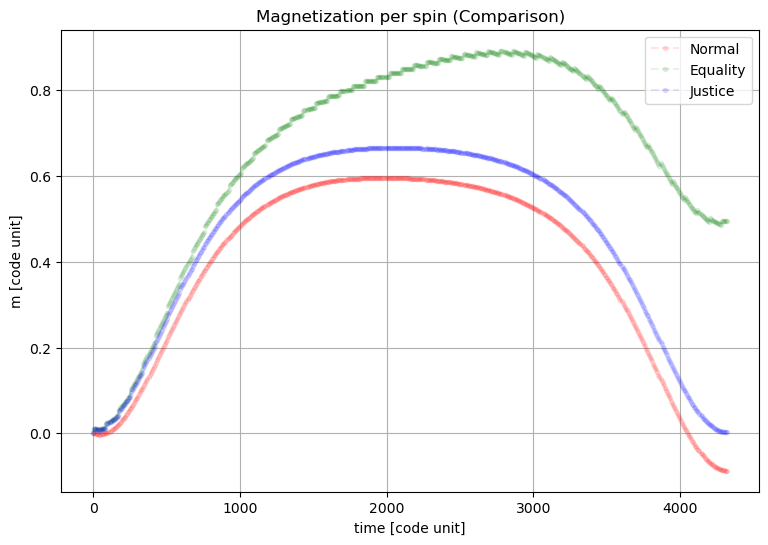
\includegraphics[width = 0.47\textwidth]{com_mt.png}
        \end{figure}
        \begin{figure}[H]
            \centering   
            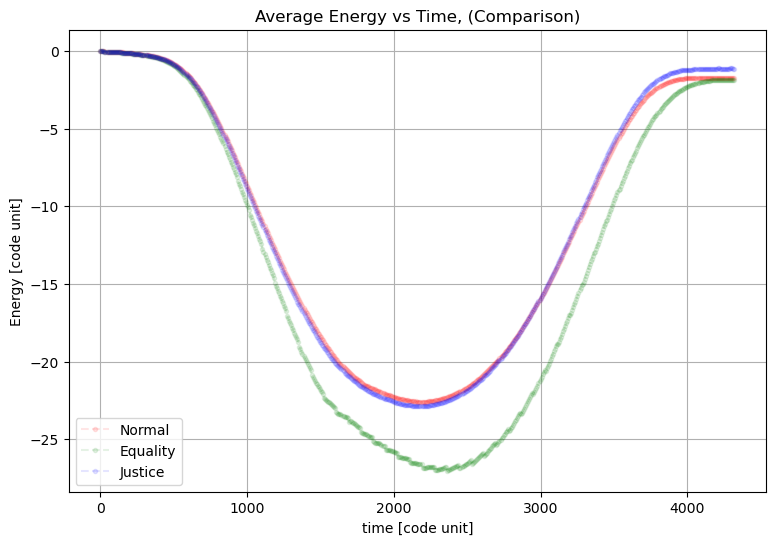
\includegraphics[width = 0.47\textwidth]{com_et.png}
            \caption{The above scheme is the magnetization per spin vs time and both of them use [code unit]. Below the energy vs time using [code unit], too. The green is Equality; the blue is justice; the red is normal. Both subsidized methods can upgrade the average ranks of the system, and lower the energy as well. Yet the equality subsidized artifice is the most significant one.}
            \label{com}
        \end{figure}
        
        Likewise, we want to investigate the system in the different phase space, here we dive into m-h space. In Figure \ref{norm_phase}, it is normal mode phase space, we first implemented the cubic spline to fit the curve, yet our system exists slopes of infinite values resulting in the first and second-order derivatives are not continuous. Therefore, we abandon the interpolated method and switch to using the curve fitting method; according to the tendency we choose reciprocal (green line, distorted) and exponential (purple line, slightly deviated. While in the literature \cite{fit}, the theoretical Ising model curve is proportional to the exponential; thus, although our simulation is not identical, we finally utilize $y = -a \times e^{(-bx + c)} + d$ to calculate susceptibility. $(a,b,c,d)$ in the above formula is the fitting free parameters. In Figure \ref{norm_phase}, implementing the green line in the above figure calculates the susceptibility in the below figure and does exist a first-order phase transition when $h \rightarrow 0$, which means that the system is sensitive when h is gradually enlarging from zero. Additionally, it is worth observing that there is a ``saturation'' magnetization, which indicates the average social rank will not arise despite the increasing external field $h$.
    \begin{figure}[H]
        \centering
        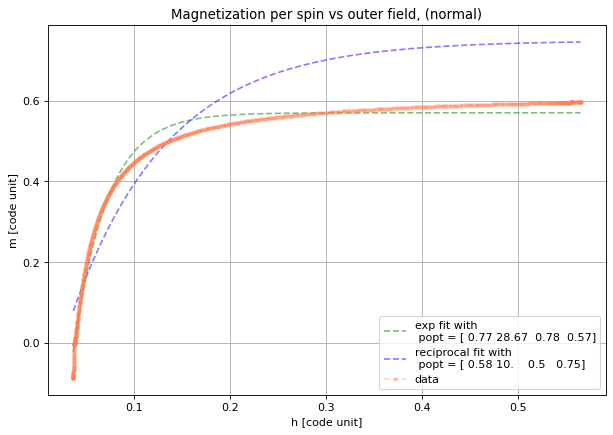
\includegraphics[width = 0.47\textwidth]{normal_mh.png} 
    \end{figure}
    \begin{figure}[H]
        \centering  
        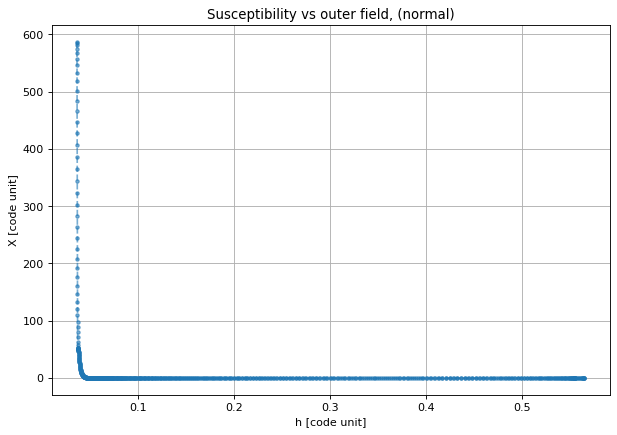
\includegraphics[width = 0.47\textwidth]{normal_Xh.png}
        \caption{The above is magnetization per spin vs external field with [code unit] with normal mode, and there presents a saturation magnetization when $h \gtrsim 0.1$. Here, we exploit two curve fitting methods, reciprocal and exponential. Lastly, we adopt the ``exponential'' method with $(a,b,c,d) \approx (0.77, 28.67, 0.78, 0.57)$. The below is the susceptibility vs external field with [code unit], and there exists a first-order phase transition when $h \rightarrow 0$.}
        \label{norm_phase}
    \end{figure}

\section{Conclusion}
    \subsection{Summary}
        The main purpose of this simulation is to research the ring model compared to the real metropolitan city with different subsidized methods. However, this is brand new research in this area under discussion, so we do not have any computational simulation reference to follow, so we take a large number of effort into the ``city comparison''. 

        In the beginning, we set up a $1000 \times 1000$ grid with random rank $[-3,3]$ and apply some exchange functions, such as the conduction function (Cond), the absorbing function of conduction (Abs.cond), the background function varies with time ($bkg\times prdc.func$), and the absorbing function of background (Abs.bkg), and combine these functions with some simulation parameters as well. In addition, so as to adhere to the idiom ``The father buys, the son builds, the grandchild sells and his son begs'', we utilize two probabilities to illustrate the poor to rich and the rich to poor situations. The results are shown in Figure \ref{2668}, \ref{overlay}. It is worth observing that there is a collapse in the middle of the grid and it presents concentric regions that almost fit the city of Burgess model such as Beijing. While the city's forming mechanism of the central zone is not completely the same as our simulation.
        
        Besides, there is a ``plateau'' in the normal mode in Figure \ref{com} (above), which means that the stable average magnetization (average social rank) will happen before reaching the lowest energy (lowest social mobility) and it will last longer than the saddle point of the energy. Moreover, investigating two subsidy policies, equality (whole ranks) and justice (rank$<1$), in our simulated condition (0.01/month, 0.02/month, respectively), the equality artifice is more efficient than the justice. Additionally, there are two characteristics in the m-h phase space, one is the saturation of magnetization and the other is the first-order phase transition. The former means this city has a maximum average social rank even though applying more external fields to the system. The latter indicates that the city is sensitive when implementing the external field (background source) gradually from zero.
   
    \subsection{Flaw}
        This project has some flaws that need to be fixed. The first is the resolution of the grid. Owing to mainly focus on observing the rank flow, we do not take population density into account, yet in a real-world situation, the population density will be an important factor. Thereby, we demand to find out more information on this part. The second is the city selection. In this project, we use Beijing as a benchmark city; yet, the city does not fully partake in the free market, so our explanation of the simulation might not absolutely fit. Hence, in order to research whether this model is reasonable or not, needing to draw on another city. The third is the temperature, in the beginning, we desired to utilize energy to deduce the temperature and it to research whether society will act the ``spontaneous polarized'' like material's spontaneous magnetization. However, we do not have a proper idea to carry out it. Additionally, in this project, we are only investigating site-background interactive, so if we have more time, it is eventful to consider the site-site interactive (i.e., correction length). On the other hand, some quantities are free parameters, we require to endow them with more meaningful explanations. Lastly, the fitting method is distorted on the saturation stage in Figure \ref{com}. We need to find a more proper way to fit it, like splitting the curve into several splines utilizing some method that can fit the infinity slopes. 
        
    \subsection{Outlook}
        In this project, we simulate a model to fit the real world, and there are more things we can study further:
        \begin{enumerate}
            \item \emph{Quantity}:
            
            Check whether our simulation fits Alonso's bid rent curve or not. Study on other parameters’ physical meaning: the background constant $B$, the experimental constants $\eta$, and the weighting of $c_{1}$ and $c_{2}$.
            
            \item \emph{Mixing backgrounds}:
            
            The background function can be any other mathematical form to simulate other sources in the real world, i.e., transportation, school, shops, etc. Also, we can apply them to multiple backgrounds to construct a more realistic situation.

            \item \emph{Extending models}:

            We can apply our simulation to other similar models with some modifications. e.g., bacterial growth in the Petri dish, behavior of wound healing, and even the analysis of plant growth and land utilization to predict house prices, etc. Since the exchange function we used in this simulation has similar physical meanings. Note that there is no minus outside the sum of differences in the conduction function for bacterial growth in the Petri dish since it's a competitive society.

            \item \emph{Exploit data to explain physical quantities more clearly}:

            Correlation length of people (rank-rank interactive), we just know that it's negatively correlated with resolution(size of grid).
 
        \end{enumerate}

\section{Acknowledgement}
    We are verily grateful to the professor for instructing us to program python with a large number of useful techniques and essential concepts of computational physics. Although this project is not near perfect, we have learned a lot of computational and collaborated skills with lustful passion! Lastly, thanks to my teammate for cooperating this final project with me!

\begin{thebibliography}{1}

    \bibitem{urban} L. Narvaez, A. Penn, S. Griffiths, Spatial Configuration and Bid Rent Theory: How urban space shapes the urban economy, ResearchGate, (2013). 
    \bibitem{fit}X. He et al. Size dependence of the magnetic properties of Nanoparticles prepared by thermal decomposition method, Nanoscale Research Letters, (2013).
    \bibitem{ring_model} Dr. Jean-Paul Rodrigue, The Burgess Urban Land Use Model, Archive.org, (2022).
    \bibitem{consentric_model} Concentric zone model, Wikipedia. (2022). 
    \bibitem{3gen}樂繼榮, 中國蘇州市吳中區西山農業園區組織人社局局長, 從富不過三代,談家風建設, (2014).
    \bibitem{mid_class}安德森, 天下雜誌: 中國的中產階級到底有多少? (2011).
    \bibitem{new}北京新生活, 在北京,生活在三環內與五環外能有多大差別, \url{https://reurl.cc/ROMx6Z}, (2018).
    \bibitem{phase_tran}Dur.ac.uk., Phase Transitions 1, \url{https://reurl.cc/rZqxGr}, (2017).
    \bibitem{price_git} liangkw16, GitHub, 北京房價分佈, \url{https://reurl.cc/kqY2bG},  (2018).
    \bibitem{toy}  Ananna Dristy, Medium, \url{https://reurl.cc/Z13MQ6}, (2021).
    
\end{thebibliography}

\end{multicols}

\clearpage

\begin{table}[]
\centering
\caption{Contribution}
\label{con}
    \begin{tabular}{c|cccc}
                                  & \textbf{Code}  & \textbf{Analysis} & \textbf{Paper} & \textbf{Slide} \\ \hline
        \textbf{City}             & Peng           & Peng(4), Ho(6)    & Peng(4), Ho(6) & Peng           \\ \hline
        \textbf{Functions}        & Peng(3), Ho(7) & Peng(5), Ho(5)    & Peng(5), Ho(5) & Peng, Ho             \\ \hline
        \textbf{Physical Analogy} & Peng           & Peng              & Peng           & Peng           \\ \hline
        \textbf{Integration}      & Peng           & Peng(6), Ho(4)    & Peng(7), Ho(3) & Peng(5), Ho(5)
    \end{tabular}
\end{table}

\section*{\Large{Codes}}
    All the codes are transferred from Jupyterlab or Python codes; therefore, if you want to rerun them, see the source code in the attached files or my GitHub repository:
    \noindent\center\url{<https://github.com/gary20000915/comphyslab-final.git>}

    \subsection*{\texttt{Prosperity\_Simulation.ipynb}}
    % do not indent if there is no indent in the source code!
        \begin{lstlisting}[language={Python}]
# %% [markdown]
# # **Common Prosperity Simulation**
# ## Computational Physics Lab 
# Authors: Yuan-Yen Peng, Chih-Tian Ho  
# E-mail: garyphys0915@gapp.nthu.edu.tw, chihtian.ho@gapp.nthu.edu.tw  
# Dept of Physics, NTHU, Taiwan   
# Date: Jan. 15, 2023  
# Version: 5.3.0 (final)      
# License: MIT

# %%
%reset -f
problem_name = 'Common_Prosperity'

# %%
import os, sys, stat
import shutil
from pathlib import Path

if os.path.exists(Path(f'./fig_{problem_name}')) == True:
    os.chmod(f'./fig_{problem_name}', stat.S_IRWXU)
    shutil.rmtree(f'./fig_{problem_name}')
    print('old folder has been removed!')

# %%
import numpy as np
from scipy.misc import derivative
from scipy.optimize import curve_fit
import matplotlib.pyplot as plt
from matplotlib.pyplot import figure
from numba import njit, prange
import time
from PIL import Image
import glob

# %% [markdown]
# ### initial conditions

# %%
# setup
io_title = problem_name
io_freq = 4 # how many steps to record the data, unit [1 month]
# unit
month = 30 # [days]
yr = 12 * month # unit: days
# size
size = int(1e3)
width, length = size, size # grid's width and length
N = int(width * length) # how many sites
tmax =  4 * 3 * yr # [days]
n = int(tmax / 7) # time steps [days]

# initial energy conditions
J = 1 # configuration constant (positive means paramagnetism)

# initial bkg condition, set the standard diviation for x & y are both 3 
SsizeE = 0.1
sigma_x, sigma_y = SsizeE * width, SsizeE * length

# intial self condition, set eta, will be adjust by results (absorbing coeff)
eta = 0.07 # absorbing rate constant

# subsidy constant for equality and justice case respectively
# quarter (Q1, Q2, Q3, Q4)  3 months = 1Q 
s_time = 3 * 4 * 7
se = int(10/10) * 0.01
sj = int(10/5) * se

# probability
p = 0.01 # rich --> poor
q = 0.01 # poor --> rich

# %% [markdown]
# ### Grid generator

# %%
def grid_generator(width, length, init_rank:float = 3.0, dec: int = 2):
  '''
  This is a grid generator
  :para width: width of the grid
  :para length: lerngth of the grid
  :para init_rank: bounds of initial rank of the grid; i.e., if use 3, --> [-3, 3]
  :para dec: decimal for the function <round>
  '''

  grid_positive = np.round(init_rank * np.random.random(int(N/2)), dec)
  grid_negative = np.round(-init_rank * np.random.random(int(N/2)), dec)
  grid = np.append(grid_positive, grid_negative)
  np.random.shuffle(grid) # set it to random
  grid = grid.reshape((width, length))

  # add the boundaries to four margins with minimum initial rank - 1
  tor = - (init_rank + 1)
  res = np.array([tor * np.ones(length)])
  grid_boundary = np.concatenate((res, grid, res), axis=0)
  grid_boundary = np.insert(grid_boundary, (0, length), tor, axis=1)

  return grid, grid_boundary

# %%
def plot(arr, header, lim, size = 8, dpi = 80):
  '''
  :para arr: input data: 2D Array
  '''

  figure(figsize=(size, size), dpi=dpi)
  plt.imshow(arr, cmap='coolwarm', extent=[-width/2,width/2,-length/2,length/2], alpha=.85)
  plt.colorbar()
  plt.clim(-lim-2.5, lim+2.5)
  plt.title(f'{header}')

  return

# %%
def plot_ct(arr, header, lim, size = 8, dpi = 80):
  '''
  :para arr: input data: 2D Array
  '''

  figure(figsize=(size, size), dpi=dpi)
  plt.imshow(arr, cmap='coolwarm', extent=[-width/2,width/2,-length/2,length/2], alpha=.75)
  plt.colorbar()
  # plt.contour(arr, colors='w', extent=[-width/2,width/2,-length/2,length/2], alpha=.85)
  plt.clim(-lim-1, lim+1)
  plt.title(f'{header}')

  return

# %% [markdown]
# ### output

# %% [markdown]
# make the directories

# %%
io_folder_fig = "fig_" + io_title
Path(io_folder_fig).mkdir(parents=True, exist_ok=True)

# %% [markdown]
# output figures

# %%
def output_fig(n, arr, lim, time, title):
  """
  Write simulation data into a file named "fig"
  """
  header = f"{title}, time = {int(time)}"
  plot(arr, header, lim)
  fig = f'{io_folder_fig}/fig_{io_title}_{title}_{str(n).zfill(3)}.png'
  plt.savefig(fig)
  plt.close() # in order to save memory

  return 

# %% [markdown]
# ### main exchange functions

# %% [markdown]
# #### Energy (each time)

# %%
@njit(parallel = True) # faster than jit if using "parallel"
def energy(spin, N, J, h):
  '''
  :para spin: is a spin matrix
  :para N: is the total number of sites
  :para J: is configuration constant (positive means paramagnetism)
  :para h: is external field
  '''

  l = int(np.sqrt(N))
  energy = np.zeros((l+2, l+2))
  for i in prange(1, l+1):
    for j in prange(1, l+1):
      s_cen  = spin[i  , j  ]
      s_up   = spin[i-1, j  ]
      s_rig  = spin[i  , j+1]
      s_down = spin[i+1, j  ]
      s_lef  = spin[i  , j-1]

      energy[i, j] = -J * s_up * s_rig * s_down * s_lef - h * s_cen

  return energy

# %% [markdown]
# #### Magnetization (each time)

# %%
def mag(spin):
  '''
  :para m: magnetization per spin (site)
  :para M: total magnetization
  '''

  M = np.sum(spin)
  m = np.average(spin)
  return m, M

# %% [markdown]
# #### Susceptibility

# %%
# @njit(parallel = True)
def X(f, h, x, size):
    dx = 1e-3
    for i in range(size):
        x[i] = derivative(f, h[i], dx)
    return x

# %% [markdown]
# #### Background function (each time)

# %%
@njit(parallel = True)
def bkg(N, sigma_x, sigma_y):
  '''
  :para N: is the total number of sites
  :para sigma_x: is a standard deviation in x-direction
  :para sigma_y: is a standard deviation in y-direction
  '''

  # l is the length; l_incluse is the length with margins; i.e., +2
  l = int(np.sqrt(N))
  l_include = l + 2
  coeff = 8e3
  BKG = np.ones((l_include, l_include))
  sigma = np.sqrt(np.square(sigma_x) + np.square(sigma_y))
  for i in prange(l):
        for j in prange(l):
            r = np.sqrt(np.square(i - l_include/2 + 2) + np.square(j - l_include/2 + 2))
            BKG[i, j] = coeff * (1/(np.sqrt(2 * np.pi) * sigma)) * (np.exp(-np.square(r) / (2 * np.square(sigma))))
  return BKG

# %% [markdown]
# #### Fitting

# %%
def func_exp(x, a, b, c, d):
  return -a * np.exp(-b * x + c) + d

def func_repo(x, a, b, c, d):
  return -a / (b*x + c) + d

# %%
def f(x, popt):
   return -popt[0] * np.exp(-popt[1] * x + popt[2]) + popt[3]

# %% [markdown]
# #### Self (spin) function (each time)

# %%
@njit(parallel = True)
def self(N, t, tmax, spin, bkg, eta):
    '''
        :para N: is the total number of sites
        :para t: is the time in the moment
        :para spin: is the spin matrix
        :para bkg: is the background function
        :para eta: absorbing rate constant

        1) set another array called new playground as nspin to save the new Hierarchy, 
            and update when all units are calculated.
        2) note that no need for bkg since they are indep. for each
    '''
    l = int(np.sqrt(N))
    nspin = np.copy(spin) # this is temp of spin (which depend on spin)
    for i in prange(1, l+1):
        for j in prange(1, l+1):

            # setup relative spins positions
            s_cen  = spin[i  , j  ]
            s_up   = spin[i-1, j  ]
            s_rig  = spin[i  , j+1]
            s_down = spin[i+1, j  ]
            s_lef  = spin[i  , j-1]

            # temp spin matrix
            nspin[i,j] += (0.5 / (3 * np.sqrt(2*np.pi)) * np.exp(-(np.square(s_cen)/(2 * np.square(3)))) * (-(4*s_cen - s_rig -s_lef - s_up - s_down))
                            + 0.5 * eta * (0.05 * np.exp(-5) * np.exp(s_cen)
                                            + (0.95 / (3 * np.sqrt(2 * np.pi))) * np.exp(-np.square(s_cen)/(2 * np.square(3)))) * bkg[i,j] * np.sin(2 * np.pi * t/tmax))
                            
            # rich --> poor
            if nspin[i,j] >= 5 and (s_rig + s_lef + s_up + s_down)/4 > 4:
                    # C are the random number [0, 1]
                    C = np.random.randint(100) / 100
                    if C <= p:
                        # the ``cross region'' will also be implicated.
                        nspin[i+1, j  ] = 0.3 * nspin[i+1, j  ] 
                        nspin[i  , j+1] = 0.3 * nspin[i  , j+1]
                        nspin[i  , j  ] = -4
                        nspin[i-1, j  ] = 0.3 * nspin[i-1, j  ]
                        nspin[i  , j-1] = 0.3 * nspin[i  , j-1]
                    else:
                        nspin[i, j] = 5
            elif nspin[i,j] >= 5 and (s_rig + s_lef + s_up + s_down)/4 <= 4:
                        nspin[i, j] = 5

            # poor --> rich
            elif nspin[i,j] <= -5 and (s_rig + s_lef + s_up + s_down)/4 < -4:
                    # C are the random number [0, 1]
                    C = np.random.randint(100) / 100
                    if C <= q:
                        nspin[i+1, j  ] = 0.3 * nspin[i+1, j  ] 
                        nspin[i  , j+1] = 0.3 * nspin[i  , j+1]
                        nspin[i  , j  ] = 4
                        nspin[i-1, j  ] = 0.3 * nspin[i-1, j  ]
                        nspin[i  , j-1] = 0.3 * nspin[i  , j-1]
                    else:
                        nspin[i, j] = -5    
            elif nspin[i,j] <= -5 and (s_rig + s_lef + s_up + s_down)/4 >= -4:
                        nspin[i, j] = -5
            # site max and min is +5 and -5

            '''
            bkg is only decay with the time (add the constraint of cos finction with the period t_max)
            '''      

            bkg[i,j] -= eta * (0.05 * np.exp(-5) * np.exp(s_cen) 
                                + (0.95 / (3 * np.sqrt(2 * np.pi))) * np.exp(-np.square(s_cen)/(2 * np.square(3)))) * bkg[i,j] * np.sin(2 * np.pi * t/tmax)

    spin = np.copy(nspin) # temp of spin = new spin (the next next matrix)

    return spin, bkg

# %% [markdown]
# #### Equality (self)

# %%
@njit(parallel = True)
def self_eq(N, t, tmax, spin, bkg, eta, se, s_time):
  '''
    :para N: is the total number of sites
    :para t: is the time in the moment
    :para spin: is the spin matrix
    :para bkg: is the background function
    :para eta: absorbing rate constant

    1) set another array called new playground as nspin to save the new Hierarchy, 
        and update when all units are calculated.
    2) note that no need for bkg since they are indep. for each
  '''
  l = int(np.sqrt(N))
  nspin = np.copy(spin) # this is temp of spin (which depend on spin)
  for i in prange(1, l+1):
      for j in prange(1, l+1):

          # setup relative spins positions
          s_cen  = spin[i  , j  ]
          s_up   = spin[i-1, j  ]
          s_rig  = spin[i  , j+1]
          s_down = spin[i+1, j  ]
          s_lef  = spin[i  , j-1]

          # temp spin matrix
          nspin[i,j] += (0.5 / (3 * np.sqrt(2*np.pi)) * np.exp(-(np.square(s_cen)/(2 * np.square(3)))) * (-(4*s_cen - s_rig -s_lef - s_up - s_down))
                                      + 0.5 * eta * (0.05 * np.exp(-5) * np.exp(s_cen)
                                              + (0.95/(3 * np.sqrt(2 * np.pi))) * np.exp(-np.square(s_cen)/(2 * np.square(3)))) * bkg[i,j] * np.sin(2 * np.pi * t/tmax))

          # Equality (all sites in [-5,5] will add se)
          # add another subsidy constant "se"
          if int(t) % s_time == 0:
            nspin[i,j] += se
            # print(f"t = {int(t)}, subsidize!")
            
          # rich --> poor
          if nspin[i,j] >= 5 and (s_rig + s_lef + s_up + s_down)/4 > 4:
                # C are the random number [0, 1]
                C = np.random.randint(100) / 100
                if C <= p:
                    # the ``cross region'' will also be implicated.
                    nspin[i+1, j  ] = 0.3 * nspin[i+1, j  ] 
                    nspin[i  , j+1] = 0.3 * nspin[i  , j+1]
                    nspin[i  , j  ] = -4
                    nspin[i-1, j  ] = 0.3 * nspin[i-1, j  ]
                    nspin[i  , j-1] = 0.3 * nspin[i  , j-1]
                else:
                    nspin[i, j] = 5
          elif nspin[i,j] >= 5 and (s_rig + s_lef + s_up + s_down)/4 <= 4:
                    nspin[i, j] = 5

          # poor --> rich
          elif nspin[i,j] <= -5 and (s_rig + s_lef + s_up + s_down)/4 < -4:
                # C are the random number [0, 1]
                C = np.random.randint(100) / 100
                if C <= q:
                        nspin[i+1, j  ] = 0.3 * nspin[i+1, j  ] 
                        nspin[i  , j+1] = 0.3 * nspin[i  , j+1]
                        nspin[i  , j  ] = 4
                        nspin[i-1, j  ] = 0.3 * nspin[i-1, j  ]
                        nspin[i  , j-1] = 0.3 * nspin[i  , j-1]
                else:
                    nspin[i, j] = -5    
          elif nspin[i,j] <= -5 and (s_rig + s_lef + s_up + s_down)/4 >= -4:
                    nspin[i, j] = -5
          # site max and min is +5 and -5

          '''
          bkg is only decay with the time (add the constraint of cos finction with the period t_max)
          '''      

          bkg[i,j] -= eta * (0.05 * np.exp(-5) * np.exp(s_cen) 
                              + (0.95 / (3 * np.sqrt(2 * np.pi))) * np.exp(-np.square(s_cen)/(2 * np.square(3)))) * bkg[i,j] * np.sin(2 * np.pi * t/tmax)

  spin = np.copy(nspin) # temp of spin = new spin (the next next matrix)

  return spin, bkg

# %% [markdown]
# #### Justice (self)

# %%
@njit(parallel = True)
def self_ju(N, t, tmax, spin, bkg, eta, sj, s_time):
  '''
    :para N: is the total number of sites
    :para t: is the time in the moment
    :para spin: is the spin matrix
    :para bkg: is the background function
    :para eta: absorbing rate constant

    1) set another array called new playground as nspin to save the new Hierarchy, 
        and update when all units are calculated.
    2) note that no need for bkg since they are indep. for each
  '''
  l = int(np.sqrt(N))
  nspin = np.copy(spin) # this is temp of spin (which depend on spin)
  for i in prange(1, l+1):
      for j in prange(1, l+1):

          # setup relative spins positions
          s_cen  = spin[i  , j  ]
          s_up   = spin[i-1, j  ]
          s_rig  = spin[i  , j+1]
          s_down = spin[i+1, j  ]
          s_lef  = spin[i  , j-1]

          # temp spin matrix
          nspin[i,j] += (0.5 / (3 * np.sqrt(2*np.pi)) * np.exp(-(np.square(s_cen)/(2 * np.square(3)))) * (-(4*s_cen - s_rig -s_lef - s_up - s_down))
                                      + 0.5 * eta * (0.05 * np.exp(-5) * np.exp(s_cen)
                                              + (0.95/(3 * np.sqrt(2 * np.pi))) * np.exp(-np.square(s_cen)/(2 * np.square(3)))) * bkg[i,j] * np.sin(2 * np.pi * t/tmax))

          # Justice (only the sites in low-class [-5,0) will add sj)
          # add another subsidy constant "sj"
          # middle class store subsidy
          if int(t) % s_time == 0:
            if nspin[i,j] < 0 and nspin[i,j] >= -5:
              nspin[i,j] += sj
              
              # if s_time == s_time:
              #   print(f"t = {int(t)}, subsidize!")
              #   break
              
          # rich --> poor
          if nspin[i,j] >= 5 and (s_rig + s_lef + s_up + s_down)/4 > 4:
                # C are the random number [0, 1]
                C = np.random.randint(100) / 100
                if C <= p:
                    # the ``cross region'' will also be implicated.
                    nspin[i+1, j  ] = 0.3 * nspin[i+1, j  ] 
                    nspin[i  , j+1] = 0.3 * nspin[i  , j+1]
                    nspin[i  , j  ] = -4
                    nspin[i-1, j  ] = 0.3 * nspin[i-1, j  ]
                    nspin[i  , j-1] = 0.3 * nspin[i  , j-1]
                else:
                    nspin[i, j] = 5
          elif nspin[i,j] >= 5 and (s_rig + s_lef + s_up + s_down)/4 <= 4:
                    nspin[i, j] = 5

          # poor --> rich
          elif nspin[i,j] <= -5 and (s_rig + s_lef + s_up + s_down)/4 < -4:
                # C are the random number [0, 1]
                C = np.random.randint(100) / 100
                if C <= q:
                        nspin[i+1, j  ] = 0.3 * nspin[i+1, j  ] 
                        nspin[i  , j+1] = 0.3 * nspin[i  , j+1]
                        nspin[i  , j  ] = 4
                        nspin[i-1, j  ] = 0.3 * nspin[i-1, j  ]
                        nspin[i  , j-1] = 0.3 * nspin[i  , j-1]
                else:
                    nspin[i, j] = -5    
          elif nspin[i,j] <= -5 and (s_rig + s_lef + s_up + s_down)/4 >= -4:
                    nspin[i, j] = -5
          # site max and min is +5 and -5

          '''
          bkg is only decay with the time (add the constraint of cos finction with the period t_max)
          '''

          bkg[i,j] -= eta * (0.05 * np.exp(-5) * np.exp(s_cen) 
                              + (0.95 / (3 * np.sqrt(2 * np.pi))) * np.exp(-np.square(s_cen)/(2 * np.square(3)))) * bkg[i,j] * np.sin(2 * np.pi * t/tmax)

  spin = np.copy(nspin) # temp of spin = new spin (the next next matrix)

  return spin, bkg

# %% [markdown]
# ### Main loop

# %%
# main (loop of time)
def main(N, n, tmax, spin, J, sigma_x, sigma_y, eta, *args):
    '''
    This is the main loop function, and it will also output the figures(.png).

    :para N: is the total number of sites
    :para n: is total number of time steps
    :para T: is the total time
    :para spin: is the spin matrix
    :para J: is configuration constant (positive means paramagnetism)
    :para sigma_x: is a standard deviation in x-direction
    :para sigma_y: is a standard deviation in y-direction
    :para eta: absorbing rate constant
    '''

    dt = 7
    t = 0
    temp_n = 0
    
    # initial setup checking 
    bk = bkg(N, sigma_x, sigma_y)
    h = 0.2 * np.average(bk) # set no bkg influences in the beginning
    Ei =energy(spin, N, J, h)
    Ei = np.delete(Ei, (0, -1), 0)
    Ei = np.delete(Ei, (0, -1), 1)
    Si = np.delete(spin, (0, -1), 0)
    Si = np.delete(Si, (0, -1), 1)
    
    m      = np.array([mag(Si)[0]])
    M      = np.array([mag(Si)[1]])
    H      = np.array([h])
    Energy = np.array([np.average(Ei)])
    
    # initial output
    clim_spin = np.max(np.abs(Si))
    clim_energy = np.max(np.abs(Ei))
    output_fig(temp_n, Si, clim_spin, t, "norm_spin")
    output_fig(temp_n, Ei, clim_energy, t, "norm_energy")
    print("Initial t = 0, succeed to output!")

    t1 = time.time()
    while t < tmax:
      # update data
      epsilon =energy(spin, N, J, h)
      spin = self(N, t, tmax, spin, bk, eta)[0]
      h = 0.2 * np.average(self(N, t, tmax, spin, bk, eta)[1])
      
      # prune margins
      S = np.delete(spin, (0, -1), 0)
      S = np.delete(S, (0, -1), 1)
      E = np.delete(epsilon, (0, -1), 0)
      E = np.delete(E, (0, -1), 1)
      
      m      = np.append(m, mag(S)[0])
      M      = np.append(M, mag(S)[1])
      H      = np.append(H, h)
      Energy = np.append(Energy, np.average(E))

      # output files
      if (temp_n % io_freq == 0):
        '''
        output info files

        '''
        output_fig(temp_n+1, S, clim_spin, t+dt, "norm_spin")
        output_fig(temp_n+1, E, clim_energy, t+dt, "norm_energy")
        print(f"{temp_n}, t = {np.round(t+dt, 2)}, succeed to output!")

      # update time and steps
      temp_n += 1
      t += dt
      if t + dt > tmax:
        dt = tmax - t

        # plot the last figure with "contour"
        # plot_ct(S, f"spin, t = {np.round(t, 2)}", clim_spin, size = 8, dpi = 80)
        # plot_ct(E, f"energy, t = {np.round(t, 2)}", clim_energy, size = 8, dpi = 80)
    t2 = time.time()
    
    # output
    T = np.linspace(0, tmax, temp_n+1)
    
    figure(figsize=(9, 6), dpi=80)
    plt.xlabel('time [code unit]')
    plt.ylabel('m [code unit]')
    plt.title(f'Magnetization per spin with {size}, (normal)')
    plt.plot(T, m, '--.', alpha = .6)
    plt.grid(True)
    plt.show()
    
    # figure(figsize=(9, 6), dpi=80)
    # plt.xlabel('time [code unit]')
    # plt.ylabel('M [code unit]')
    # plt.title(f'Magnetization with {size}')
    # plt.plot(T, M, '--.', alpha = .6)
    # plt.grid(True)
    # plt.show()
    
    figure(figsize=(9, 6), dpi=80)
    plt.xlabel('time [code unit]')
    plt.ylabel('Energy [code unit]')
    plt.title(f'Average Energy vs Time, (normal)')
    plt.plot(T, Energy, '--.', alpha = .6)
    plt.grid(True)
    plt.show()
    
    HH = np.sort(H, axis=None)
    mm = np.sort(m, axis=None)

    xdata = HH
    ydata = mm
    
    # fitting m-h
    popt, pcov = curve_fit(func_exp, xdata, ydata, bounds=(-0.5, [2., 50., 2., 1.]))
    popt_, pcov_ = curve_fit(func_repo, xdata, ydata, bounds=(0.5, [2., 10., 2., 1.]), p0=([2,5,1,0.6])) 
    
    figure(figsize=(9, 6), dpi=80)
    plt.xlabel('h [code unit]')
    plt.ylabel('m [code unit]')
    plt.title(f'Magnetization per spin vs outer field, (normal)')
    plt.plot(xdata, func_exp(xdata, *popt), '--g', alpha = .5, label = f'exp fit with \n popt = {np.round(popt, 2)}')
    plt.plot(xdata, func_exp(xdata, *popt_), '--b', alpha = .5, label = f'reciprocal fit with \n popt = {np.round(popt_,2)}')
    plt.plot(HH, mm, '--.', color = 'coral', alpha = .3, label='data')
    plt.legend()
    plt.grid(True)
    plt.show()

    x = np.zeros(np.size(mm)-1)
    x_size = int(np.size(x))
    def f(x):
      return -popt[0] * np.exp(-popt[1] * x + popt[2]) + popt[3]
    xx = X(f, ydata, x, x_size)
    HH = np.delete(HH, [-1], axis=0)
    figure(figsize=(9, 6), dpi=80)
    plt.xlabel('h [code unit]')
    plt.ylabel('X [code unit]')
    plt.title(f'Susceptibility vs outer field, (normal)')
    plt.plot(HH, xx, '--.', alpha = .6)
    plt.grid(True)
    plt.show()
    
    return print("Done! Time = ", np.round(t2 - t1, 3), "[s]"), T, m, T, Energy

# %% [markdown]
# #### main equality

# %%
# main (loop of time)
def main_e(N, n, tmax, spin, J, sigma_x, sigma_y, eta, *args):
    '''
    This is the main loop function, and it will also output the figures(.png).

    :para N: is the total number of sites
    :para n: is total number of time steps
    :para T: is the total time
    :para spin: is the spin matrix
    :para J: is configuration constant (positive means paramagnetism)
    :para sigma_x: is a standard deviation in x-direction
    :para sigma_y: is a standard deviation in y-direction
    :para eta: absorbing rate constant
    '''

    dt = 7
    t = 0
    temp_n = 0
    
    # initial setup checking 
    bk = bkg(N, sigma_x, sigma_y)
    h = 0.2 * np.average(bk) # set no bkg influences in the beginning
    Ei =energy(spin, N, J, h)
    Ei = np.delete(Ei, (0, -1), 0)
    Ei = np.delete(Ei, (0, -1), 1)
    Si = np.delete(spin, (0, -1), 0)
    Si = np.delete(Si, (0, -1), 1)
    
    m      = np.array([mag(Si)[0]])
    M      = np.array([mag(Si)[1]])
    H      = np.array([h])
    Energy = np.array([np.average(Ei)])
    
    # initial output
    clim_spin = np.max(np.abs(Si))
    clim_energy = np.max(np.abs(Ei))
    output_fig(temp_n, Si, clim_spin, t, "eq_spin")
    output_fig(temp_n, Ei, clim_energy, t, "eq_energy")
    print("Initial t = 0, succeed to output!")

    t1 = time.time()
    while t < tmax:
      # update data
      epsilon =energy(spin, N, J, h)
      spin = self_eq(N, t, tmax, spin, bk, eta, se, s_time)[0]
      h = 0.2 * np.average(self_eq(N, t, tmax, spin, bk, eta, se, s_time)[1])
      
      # prune margins
      S = np.delete(spin, (0, -1), 0)
      S = np.delete(S, (0, -1), 1)
      E = np.delete(epsilon, (0, -1), 0)
      E = np.delete(E, (0, -1), 1)
      
      m      = np.append(m, mag(S)[0])
      M      = np.append(M, mag(S)[1])
      H      = np.append(H, h)
      Energy = np.append(Energy, np.average(E))

      # output files
      if (temp_n % io_freq == 0):
        '''
        output info files

        '''
        output_fig(temp_n+1, S, clim_spin, t+dt, "eq_spin")
        output_fig(temp_n+1, E, clim_energy, t+dt, "eq_energy")
        print(f"{temp_n}, t = {np.round(t+dt, 2)}, succeed to output!")

      # update time and steps
      temp_n += 1
      t += dt
      if t + dt > tmax:
        dt = tmax - t

        # plot the last figure with "contour"
        # plot_ct(S, f"spin, t = {np.round(t, 2)}", clim_spin, size = 8, dpi = 80)
        # plot_ct(E, f"energy, t = {np.round(t, 2)}", clim_energy, size = 8, dpi = 80)
    t2 = time.time()
    
    # output
    T = np.linspace(0, tmax, temp_n+1)
    
    figure(figsize=(9, 6), dpi=80)
    plt.xlabel('time [code unit]')
    plt.ylabel('m [code unit]')
    plt.title(f'Magnetization per spin with {size}, (Equality)')
    plt.plot(T, m, '--.', alpha = .6)
    plt.grid(True)
    plt.show()
    
    # figure(figsize=(9, 6), dpi=80)
    # plt.xlabel('time [code unit]')
    # plt.ylabel('M [code unit]')
    # plt.title(f'Magnetization with {size}')
    # plt.plot(T, M, '--.', alpha = .6)
    # plt.grid(True)
    # plt.show()
    
    figure(figsize=(9, 6), dpi=80)
    plt.xlabel('time [code unit]')
    plt.ylabel('Energy [code unit]')
    plt.title(f'Average Energy vs Time, (Equality)')
    plt.plot(T, Energy, '--.', alpha = .6)
    plt.grid(True)
    plt.show()
    
    HH = np.sort(H, axis=None)
    mm = np.sort(m, axis=None)

    # fitting m-h
    xdata, ydata = HH, mm
    popt, pcov = curve_fit(func_exp, xdata, ydata, bounds=(-0.5, [2., 50., 2., 1.]))
    popt_, pcov_ = curve_fit(func_repo, xdata, ydata, bounds=(0.5, [2., 10., 1., 1.]), p0=([2,5,1,0.6])) 

    figure(figsize=(9, 6), dpi=80)
    plt.xlabel('h [code unit]')
    plt.ylabel('m [code unit]')
    plt.title(f'Magnetization per spin vs outer field, (Equality)')
    plt.plot(xdata, func_exp(xdata, *popt), '--g', alpha = .5, label = f'exp fit with \n popt = {np.round(popt, 2)}')
    plt.plot(xdata, func_exp(xdata, *popt_), '--b', alpha = .5, label = f'reciprocal fit with \n popt = {np.round(popt_,2)}')
    plt.plot(HH, mm, '--.', color = 'coral', alpha = .3, label='data')
    plt.legend()
    plt.grid(True)
    plt.show()

    x = np.zeros(np.size(mm)-1)
    x_size = int(np.size(x))
    def f(x):
      return -popt[0] * np.exp(-popt[1] * x + popt[2]) + popt[3]
    xx = X(f, ydata, x, x_size)
    HH = np.delete(HH, [-1], axis=0)
    figure(figsize=(9, 6), dpi=80)
    plt.xlabel('h [code unit]')
    plt.ylabel('X [code unit]')
    plt.title(f'Susceptibility vs outer field, (Equality)')
    plt.plot(HH, xx, '--.', alpha = .6)
    plt.grid(True)
    plt.show()
    
    return print("Done! Time = ", np.round(t2 - t1, 3), "[s]"), T, m, T, Energy

# %% [markdown]
# #### main justice

# %%
# main (loop of time)
def main_j(N, n, tmax, spin, J, sigma_x, sigma_y, eta, *args):
    '''
    This is the main loop function, and it will also output the figures(.png).

    :para N: is the total number of sites
    :para n: is total number of time steps
    :para T: is the total time
    :para spin: is the spin matrix
    :para J: is configuration constant (positive means paramagnetism)
    :para sigma_x: is a standard deviation in x-direction
    :para sigma_y: is a standard deviation in y-direction
    :para eta: absorbing rate constant
    '''

    dt = 7
    t = 0
    temp_n = 0
    
    # initial setup checking 
    bk = bkg(N, sigma_x, sigma_y)
    h = 0.2 * np.average(bk) # set no bkg influences in the beginning
    Ei =energy(spin, N, J, h)
    Ei = np.delete(Ei, (0, -1), 0)
    Ei = np.delete(Ei, (0, -1), 1)
    Si = np.delete(spin, (0, -1), 0)
    Si = np.delete(Si, (0, -1), 1)
    
    m      = np.array([mag(Si)[0]])
    M      = np.array([mag(Si)[1]])
    H      = np.array([h])
    Energy = np.array([np.average(Ei)])
    
    # initial output
    clim_spin = np.max(np.abs(Si))
    clim_energy = np.max(np.abs(Ei))
    output_fig(temp_n, Si, clim_spin, t, "ju_spin")
    output_fig(temp_n, Ei, clim_energy, t, "ju_energy")
    print("Initial t = 0, succeed to output!")

    t1 = time.time()
    while t < tmax:
      # update data
      epsilon =energy(spin, N, J, h)
      spin = self_ju(N, t, tmax, spin, bk, eta, sj, s_time)[0]
      h = 0.2 * np.average(self_eq(N, t, tmax, spin, bk, eta, sj, s_time)[1])
      
      # prune margins
      S = np.delete(spin, (0, -1), 0)
      S = np.delete(S, (0, -1), 1)
      E = np.delete(epsilon, (0, -1), 0)
      E = np.delete(E, (0, -1), 1)
      
      m      = np.append(m, mag(S)[0])
      M      = np.append(M, mag(S)[1])
      H      = np.append(H, h)
      Energy = np.append(Energy, np.average(E))

      # output files
      if (temp_n % io_freq == 0):
        '''
        output info files

        '''
        output_fig(temp_n+1, S, clim_spin, t+dt, "ju_spin")
        output_fig(temp_n+1, E, clim_energy, t+dt, "ju_energy")
        print(f"{temp_n}, t = {np.round(t+dt, 2)}, succeed to output!")

      # update time and steps
      temp_n += 1
      t += dt
      if t + dt > tmax:
        dt = tmax - t

        # plot the last figure with "contour"
        # plot_ct(S, f"spin, t = {np.round(t, 2)}", clim_spin, size = 8, dpi = 80)
        # plot_ct(E, f"energy, t = {np.round(t, 2)}", clim_energy, size = 8, dpi = 80)
    t2 = time.time()
    
    # output
    T = np.linspace(0, tmax, temp_n+1)
    
    figure(figsize=(9, 6), dpi=80)
    plt.xlabel('time [code unit]')
    plt.ylabel('m [code unit]')
    plt.title(f'Magnetization per spin with {size}, (Justice)')
    plt.plot(T, m, '--.', alpha = .6)
    plt.grid(True)
    plt.show()
    
    # figure(figsize=(9, 6), dpi=80)
    # plt.xlabel('time [code unit]')
    # plt.ylabel('M [code unit]')
    # plt.title(f'Magnetization with {size}')
    # plt.plot(T, M, '--.', alpha = .6)
    # plt.grid(True)
    # plt.show()
    
    figure(figsize=(9, 6), dpi=80)
    plt.xlabel('time [code unit]')
    plt.ylabel('Energy [code unit]')
    plt.title(f'Average Energy vs Time, (Justice)')
    plt.plot(T, Energy, '--.', alpha = .6)
    plt.grid(True)
    plt.show()
    
    HH = np.sort(H, axis=None)
    mm = np.sort(m, axis=None)

    xdata, ydata = HH, mm
    popt, pcov = curve_fit(func_exp, xdata, ydata, bounds=(-0.5, [2., 50., 2., 1.]))
    popt_, pcov_ = curve_fit(func_repo, xdata, ydata, bounds=(0.5, [2., 10., 2., 1.]), p0=([2,5,1,0.6])) 

    figure(figsize=(9, 6), dpi=80)
    plt.xlabel('h [code unit]')
    plt.ylabel('m [code unit]')
    plt.title(f'Magnetization per spin vs outer field, (Justice)')
    plt.plot(xdata, func_exp(xdata, *popt), '--g', alpha = .5, label = f'exp fit with \n popt = {np.round(popt, 2)}')
    plt.plot(xdata, func_exp(xdata, *popt_), '--b', alpha = .5, label = f'reciprocal fit with \n popt = {np.round(popt_,2)}')
    plt.plot(HH, mm, '--.', color = 'coral', alpha = .3, label='data')
    plt.legend()
    plt.grid(True)
    plt.show()
    
    x = np.zeros(np.size(mm)-1)
    x_size = int(np.size(x))
    def f(x):
      return -popt[0] * np.exp(-popt[1] * x + popt[2]) + popt[3]
    xx = X(f, ydata, x, x_size)
    HH = np.delete(HH, [-1], axis=0)
    figure(figsize=(9, 6), dpi=80)
    plt.xlabel('h [code unit]')
    plt.ylabel('X [code unit]')
    plt.title(f'Susceptibility vs outer field, (Justice)')
    plt.plot(HH, xx, '--.', alpha = .6)
    plt.grid(True)
    plt.show()

    return print("Done! Time = ", np.round(t2 - t1, 3), "[s]"), T, m, T, Energy

# %% [markdown]
# ### Execution

# %%
'''
main for normal loop
'''
print("Norm \n")
t1 = time.time()
spin = grid_generator(width, length, init_rank = 3.0, dec = 2)[1] # include boundary
norm = main(N, n, tmax, spin, J, sigma_x, sigma_y, eta)
x_norm, y_norm = norm[1], norm[2]
X_norm, Y_norm = norm[3], norm[4]
t2 = time.time()

print(f"Taking {np.round((t2 - t1), 3)} [s]")
print("Finish!")

# %%
'''
main loop of equality
'''
print("Eq \n")
t1 = time.time()
spin = grid_generator(width, length, init_rank = 3.0, dec = 2)[1] # include boundary
eq = main_e(N, n, tmax, spin, J, sigma_x, sigma_y, eta, se, s_time)
x_eq, y_eq = eq[1], eq[2]
X_eq, Y_eq = eq[3], eq[4]
t2 = time.time()

print(f"Taking {np.round((t2 - t1), 3)} [s]")
print("Finish!")

# %%
'''
main loop of jutice
'''
print("Ju \n")
t1 = time.time()
spin = grid_generator(width, length, init_rank = 3.0, dec = 2)[1] # include boundary
j = main_j(N, n, tmax, spin, J, sigma_x, sigma_y, eta, se, s_time)
x_j, y_j = j[1], j[2]
X_j, Y_j = j[3], j[4]
t2 = time.time()

print(f"Taking {np.round((t2 - t1), 3)} [s]")
print("Finish!")

# %% [markdown]
# ##### Comparison printing

# %%
# m vs t
figure(figsize=(9, 6), dpi=100)
plt.xlabel('time [code unit]')
plt.ylabel('m [code unit]')
plt.title(f'Magnetization per spin (Comparison)')
plt.plot(x_norm, y_norm, '--.', color='r', alpha = .1, label='Normal')
plt.plot(x_eq, y_eq, '--.', color='g', alpha = .1, label='Equality')
plt.plot(x_j, y_j, '--.', color='b', alpha = .1, label='Justice')
plt.grid(True)
plt.legend()
plt.show()

# %%
# E vs t
figure(figsize=(9, 6), dpi=100)
plt.xlabel('time [code unit]')
plt.ylabel('Energy [code unit]')
plt.title(f'Average Energy vs Time, (Comparison)')
plt.plot(X_norm, Y_norm, '--.', color='r', alpha = .1, label='Normal')
plt.plot(X_eq, Y_eq, '--.', color='g', alpha = .1, label='Equality')
plt.plot(X_j, Y_j, '--.', color='b', alpha = .1, label='Justice')
plt.grid(True)
plt.legend()
plt.show()

# %% [markdown]
# ### Creat GIF

# %%
'''
eq spin
'''

# Create the frames
frames = []
imgs = glob.glob(f"{io_folder_fig}/fig_Common_Prosperity_eq_spin_*.png")
imgs.sort()
# check the sorted result
print(imgs)

for i in imgs:
    new_frame = Image.open(i)
    frames.append(new_frame)

# Save into a GIF file that loops forever
frames[0].save('eq_spin.gif', format='GIF',
                append_images=frames[1:],
                save_all=True,
                duration=200, loop=0)

print("Done!")

# %%
'''
jutice spin
'''

# Create the frames
frames = []
imgs = glob.glob(f"{io_folder_fig}/fig_Common_Prosperity_ju_spin_*.png")
imgs.sort()
# check the sorted result
print(imgs)

for i in imgs:
    new_frame = Image.open(i)
    frames.append(new_frame)

# Save into a GIF file that loops forever
frames[0].save('ju_spin.gif', format='GIF',
                append_images=frames[1:],
                save_all=True,
                duration=200, loop=0)

print("Done!")

# %%
'''
norm spin
'''

# Create the frames
frames = []
imgs = glob.glob(f"{io_folder_fig}/fig_Common_Prosperity_norm_spin_*.png")
imgs.sort()
# check the sorted result
print(imgs)

for i in imgs:
    new_frame = Image.open(i)
    frames.append(new_frame)

# Save into a GIF file that loops forever
frames[0].save('norm_spin.gif', format='GIF',
                append_images=frames[1:],
                save_all=True,
                duration=200, loop=0)

print("Done!")

# %%
# '''
# Energy
# '''

# # Create the frames
# frames = []
# imgs = glob.glob(f"{io_folder_fig}/fig_Common_Prosperity_norm_energy_*.png")
# imgs.sort()
# # check the sorted result
# print(imgs)

# for i in imgs:
#     new_frame = Image.open(i)
#     frames.append(new_frame)

# # Save into a GIF file that loops forever
# frames[0].save('energy.gif', format='GIF',
#                 append_images=frames[1:],
#                 save_all=True,
#                 duration=300, loop=0)

# print("Done!")



        \end{lstlisting}


\end{document}